
\chapter{Estado de la cuestión}
El desarrollo de sistemas de gestión y monitorización de documentos es un área de gran relevancia en el ámbito empresarial, especialmente en sectores donde la integridad y disponibilidad de la información son críticas. En este capítulo, se analiza el impacto de la pérdida de documentos, las iniciativas existentes para su monitorización y las tecnologías web más utilizadas en la actualidad.

Aquí tienes la sección ampliada con los cambios solicitados, incorporando mayor detalle y referencias bibliográficas:


\section{Impacto y costes de la pérdida de documentos}
La gestión documental efectiva constituye un pilar fundamental en la operativa empresarial moderna, donde la digitalización y el volumen de información generada plantean desafíos crecientes. Una gestión inadecuada puede desencadenar consecuencias devastadoras tanto a nivel operativo como legal y reputacional.

\subsection{Riesgos en el ciclo de vida documental}
El proceso de gestión de documentos implica múltiples etapas críticas donde pueden producirse fallos. Según \citetitle{ISO15801:2017}, hasta el 43\% de las pérdidas documentales ocurren durante las fases de transferencia o almacenamiento temporal. Un riesgo particular surge cuando la generación de documentos se delega a proveedores externos, práctica común en sectores como el legal. Este outsourcing introduce vulnerabilidades al:

\begin{itemize}
    \item Multiplicar los puntos de contacto en el flujo documental
    \item Requerir protocolos de transferencia seguros entre sistemas heterogéneos
    \item Dificultar la auditoría de trazabilidad completa
\end{itemize}

\subsection{Consecuencias operativas y regulatorias}
En el ámbito empresarial, la falta de acceso a información crítica genera interrupciones en cadena. Los costes asociados, como detalla el informe \citetitle{IBM2024}, incluyen:

\begin{itemize}
    \item Costes directos de recuperación (€35.000-€250.000 por incidente)
    \item Multas regulatorias (hasta 4\% del volumen de negocio anual bajo GDPR)
    \item Litigios por incumplimiento contractual
\end{itemize}

Sectores regulados como el bancario o sanitario enfrentan riesgos amplificados. La pérdida de documentos que contengan datos personales compromete no solo la privacidad, sino que genera responsabilidades legales escalonadas. El análisis de \textcite{cost-doc-manag-2020} revela que el 23\% de las brechas en estos sectores se originan en fallos de gestión documental, con costes medios por registro comprometido entre €350-€700.


\section{Otras iniciativas}
Ante la necesidad de garantizar la disponibilidad y seguridad de los documentos, se han desarrollado diversas iniciativas para su monitorización y gestión. Entre las más comunes se encuentran:

\begin{itemize}
    \item \textbf{Soluciones Open Source }: Dos de las aplicaciones Open Source más conocidas para la gestión de documentos son Alfresco y OpenKM.
    Alfresco es un sistema de gestión documental open source desarrollado en Java. Su versión Community es gratuita pero requiere especialistas para su implementación. Aunque ofrece potentes APIs de integración, su versión Enterprise tiene costos prohibitivos para medianas empresas \parencite{Evoltia2023}. 
    Por otro lado cabe destacar que las soluciones open source preexistentes requieren conocimientos técnicos avanzados para su implementación y mantenimiento.
    
    Por otro lado, OpenKM es una plataforma libre con interfaz web basada en tecnologías Java. Su versión Community sigue el modelo GPLv2, pero las versiones Professional y Cloud son comerciales. Aunque ofrece búsqueda avanzada y flujos de trabajo, su escalabilidad en entornos complejos es limitada \parencite{OpenKM2023}.
    
    \item Plataformas cloud comerciales (OneDrive/Google Drive):
    Soluciones SaaS fáciles de implementar pero con limitaciones en control de datos, cumplimiento normativo para sectores regulados y dependencia del proveedor. Carecen de funcionalidades avanzadas de gestión documental como workflows complejos o metadata estructurada. La principal desventaja de las plataformas cloud comerciales es que carecen de control sobre los datos y no cumplen con regulaciones estrictas.

    \item Sistemas de monitorización mediante scripts: Soluciones basadas en scripts personalizados que verifican el estado de los documentos en una base de datos. Aunque son flexibles y de bajo coste, su mantenimiento puede ser complejo y no suelen escalar bien en entornos con grandes volúmenes de datos.
    
    \item Bases de datos duplicadas: Estrategia que consiste en mantener copias redundantes de los documentos en diferentes servidores. Aunque mejora la disponibilidad, implica un mayor coste de almacenamiento y puede complicar la sincronización entre las bases de datos.
    
    \item Consultas \acrshort{sql} básicas: Uso de consultas \acrfull{sql} para verificar el estado de los documentos. Esta aproximación es sencilla pero limitada, ya que no ofrece funcionalidades avanzadas como la generación de informes o la integración con otras herramientas.
\end{itemize}

Estas iniciativas, aunque útiles en ciertos contextos, presentan limitaciones en términos de escalabilidad, seguridad y facilidad de uso, lo que justifica la necesidad de soluciones más avanzadas como SIDManager.

%--------------------------
\section{Tecnologías web}
%--------------------------
El desarrollo de aplicaciones web modernas requiere la selección de tecnologías adecuadas que permitan construir sistemas eficientes, seguros y escalables.

En este contexto, conviene distinguir entre un script y una aplicación web. Un \emph{script} es un conjunto de instrucciones escritas en un lenguaje de programación (como Python o bash) que se ejecutan de manera secuencial para realizar tareas específicas. Aunque son útiles para automatizar procesos, los scripts suelen carecer de una interfaz de usuario y no están diseñados para manejar grandes volúmenes de datos o usuarios concurrentes.

En cambio, una \emph{aplicación web} \parencite{AWS2025} es un sistema completo que incluye una interfaz de usuario, lógica de negocio y persistencia de datos. Las aplicaciones web están diseñadas para ser accesibles desde navegadores y suelen utilizar tecnologías como \acrfull{html}, \acrfull{css}, JavaScript en el front-end, y frameworks como Spring Boot o Django en el backend. A diferencia de los scripts, las aplicaciones web son escalables, seguras y ofrecen una experiencia de usuario más completa.
En este capítulo  se analizan las tecnologías más relevantes en este último ámbito.
 

\subsection{Metodos HTTP }

Como sostiene la \textcite{MDN_HTTP_Methods}, los métodos HTTP (HyperText Transfer Protocol) son la base de la comunicación en la web y definen las operaciones que se pueden realizar sobre los recursos. Los más utilizados son los métodos \acrshort{get} y los métodos \acrshort{post}.

Un método GET se utiliza para solicitar datos de un recurso específico. Es idempotente, lo que significa que múltiples solicitudes GET no modifican el estado del servidor. Este método es ideal para recuperar información, como listados de documentos o detalles de un usuario.

Por contra, un
método POST se utiliza para enviar datos al servidor, generalmente para crear nuevos recursos. A diferencia de GET, POST no es idempotente, ya que cada solicitud puede generar un cambio en el servidor. Este método es común en formularios de registro o envío de datos.

\subsection{API}
Una \acrfull{api} es un conjunto de reglas y protocolos que permite la comunicación entre diferentes sistemas. Las APIs son fundamentales en el desarrollo de aplicaciones modernas, ya que facilitan la integración entre servicios y permiten construir sistemas modulares y escalables.

\subsection{REST}
\acrfull{rest} es un estilo arquitectónico para diseñar APIs web. Se basa en el uso de métodos HTTP (GET, POST, \acrshort{put}, DELETE) para realizar operaciones sobre recursos identificados por \acrshort{url}s. REST es ampliamente utilizado debido a su simplicidad, escalabilidad y compatibilidad con diferentes tecnologías. Además, las APIs RESTful son fáciles de consumir desde clientes web, móviles o de escritorio, lo que las convierte en una opción ideal para aplicaciones como SIDManager.


\section{Herramientas para el desarrollo }

En este capítulo se describen las principales tecnologías y herramientas utilizadas en el desarrollo de esta aplicación web, analizando su origen, propósito y cómo contribuyen al proyecto.

\subsection{Angular}

Tal y como explica \textcite{Zurawski2024}, Angular 
es un framework de desarrollo web creado por Google en 2010, diseñado para facilitar la construcción de aplicaciones de una sola página (\acrshort{spa}) en el lado del cliente. Estaba basado en JavaScript, así se ve en \citetitle{javascript} de \citeauthor{javascript}
 pero desde la versión 2, tanto internamente en la aplicación como para hacer desarrollos con esta, se utiliza TypeScript \parencite{typescript}
 un superconjunto de JavaScript que añade tipado estático, mejorando la robustez y escalabilidad de las aplicaciones desarrolladas con Angular.
El principal propósito de Angular es simplificar la creación de interfaces de usuario dinámicas y reactivas, permitiendo que los desarrolladores gestionen el contenido de forma más eficiente. Su arquitectura basada en componentes y el uso de un sistema de inyección de dependencias hacen que Angular sea muy adecuado para grandes aplicaciones front-end. Además, ofrece un sistema de dos vías de enlace de datos (two-way data binding) que sincroniza de manera automática los cambios entre el modelo y la vista.

\begin{figure}
    \centering
    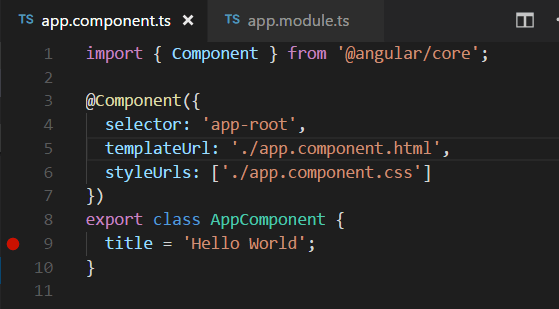
\includegraphics[width=0.75\linewidth]{imagenes/code/angular_components.png}
    \caption{Ejemplo de componentes de Angular con código Typescript. }
    \label{fig:angular_components}
\end{figure}

Angular es parte de un conjunto más amplio de herramientas y tecnologías de Google, por lo que su integración con otros servicios de Google es fluida. A lo largo de los años, ha ganado popularidad en el desarrollo front-end, especialmente en entornos empresariales, debido a su capacidad para manejar aplicaciones de gran escala y su enfoque en la modularidad y reutilización de código.

Uno de los lenguajes que se utiliza en Angular es TypeScript, que proporciona características de programación orientada a objetos como clases, interfaces y herencia, facilitando el desarrollo de aplicaciones más mantenibles. Este lenguaje lo hace ideal para proyectos de gran tamaño, donde el control de tipos puede ayudar a reducir errores. A pesar de ser un framework basado en el front-end, Angular puede integrarse con varios backends, como Node.js, Django, Spring, entre otros.

Angular es un framework respaldado por Google, lo que asegura un ciclo de vida estable y una comunidad activa que contribuye a su mejora continua. Además, dado que Angular es open-source, la comunidad también juega un papel clave en su evolución, lo que garantiza que el framework continúe siendo relevante en la industria del desarrollo web.

Aunque Angular es muy popular, su curva de aprendizaje puede ser algo pronunciada, especialmente para desarrolladores novatos. Además, debido a su carácter completo, puede ser excesivo para aplicaciones más pequeñas, donde un framework más ligero podría ser suficiente. Sin embargo, en proyectos de gran escala que requieren una estructura bien organizada y mantenible, Angular sigue siendo una opción sólida.

\subsection{React}
React es una biblioteca de JavaScript para la construcción de interfaces de usuario, desarrollada por Facebook (ahora Meta), como se puede apreciar en el artículo \citetitle{facebook},
y lanzada al público en 2013. Su principal propósito es facilitar el desarrollo de aplicaciones web interactivas y reactivas mediante un enfoque basado en componentes reutilizables. 

React se enfoca en la parte de la vista (view) en el patrón de diseño 
\acrfull{mvc} como explica \citeauthor{MVC} en el estudio \citetitle{MVC}, lo que permite crear interfaces dinámicas sin tener que recargar la página web.

Una de las características más destacadas de React es su uso del \acrfull{vdom} tal y como explica en \citetitle{virtual-dom}. Este artículo sostiene que se obtiene una mejora significativa en el rendimiento al minimizar la manipulación directa del DOM del navegador. En lugar de modificar el DOM completo con cada cambio, React crea una copia de este en memoria y solo actualiza las partes que han cambiado, lo que hace que las aplicaciones sean más rápidas y eficientes.

\begin{figure}
    \centering
    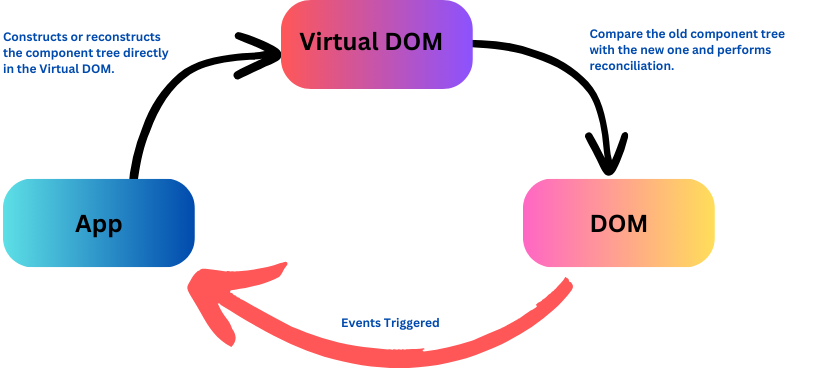
\includegraphics[width=0.75\linewidth]{imagenes/scheme/react_virtual_dom.png}
    \caption{Ejemplo de DOM virtual de React hecho por \textcite{virtual-dom-scheme}}
    \label{fig:react_virtual_dom}
\end{figure}

React está escrito en JavaScript, pero con soporte extendido para \acrfull{jsx} (para más información, ver el informe de \citeauthor{JSX} llamado \citetitle{JSX})
una extensión de sintaxis que permite escribir elementos de la interfaz de usuario de forma declarativa, como si fueran parte del código HTML. Esto facilita a los desarrolladores visualizar claramente la estructura del componente dentro del código JavaScript, simplificando el desarrollo y mantenimiento de la interfaz.

El ecosistema de React ha crecido enormemente desde su lanzamiento. Aunque originalmente fue concebido para aplicaciones de una sola página (SPA), React ha evolucionado para ser usado tanto en el desarrollo front-end como en aplicaciones móviles, mediante el uso de React Native. Esto convierte a React en una tecnología versátil, usada en una amplia variedad de plataformas.

Una ventaja importante de React es su flexibilidad: no impone una arquitectura rígida y se puede integrar fácilmente con otras bibliotecas o frameworks. 

A pesar de sus ventajas, React tiene algunas desventajas. Una de ellas es que, aunque es fácil de aprender para pequeños proyectos, gestionar el estado en aplicaciones grandes puede volverse complicado, lo que requiere el uso de bibliotecas externas como Redux o Context API. Además, React es solo una biblioteca para la vista, lo que significa que carece de muchas funcionalidades de un framework completo, como el enrutamiento o la gestión de dependencias, que deben añadirse manualmente.

React ha ganado una enorme popularidad desde su lanzamiento y sigue siendo una de las bibliotecas más utilizadas para el desarrollo web, debido a su eficiencia, flexibilidad y soporte por parte de una comunidad muy activa.

\subsection{ Spring }
Spring es un marco de trabajo (framework) para el desarrollo de aplicaciones en Java, como sostiene \cite{spring-def}
, ampliamente utilizado en entornos empresariales debido a su flexibilidad y capacidad para facilitar el desarrollo de aplicaciones robustas y escalables. Fue desarrollado por Rod Johnson y lanzado inicialmente en 2003, como una alternativa ligera a los frameworks Java más pesados de la época. Spring permite construir aplicaciones que siguen los principios de inyección de dependencias y programación orientada a aspectos (para más detalle sobre programación orientada a objetos ver \textcite{aop})
, lo que mejora la modularidad y facilita la gestión de la complejidad en proyectos grandes.



El propósito principal de Spring es simplificar el desarrollo de aplicaciones en Java, proporcionando una infraestructura sólida que resuelve los problemas comunes en la creación de aplicaciones de servidor. Además de su flexibilidad, Spring se destaca por sus capacidades de integración con otros frameworks y tecnologías, lo que lo convierte en una solución versátil para la creación de aplicaciones web, \gls{api}
y microservicios.

Spring es el framework base que se extiende a través de módulos como Spring MVC (para aplicaciones web), Spring Security (para control de acceso) y Spring Data (para gestión de bases de datos). Gracias a su popularidad, sigue siendo el framework Java más utilizado para el desarrollo de aplicaciones empresariales.

\subsection{ Spring Boot }
Spring Boot es una extensión del framework Spring que fue publicada en 2014 por Pivotal Software. Está diseñada para simplificar el proceso de configuración y arranque de las aplicaciones desarrolladas en Spring. Mientras que Spring ofrece una gran flexibilidad, su configuración puede ser tediosa y propensa a errores. Aquí es donde Spring Boot aporta su valor: reduce la necesidad de configuración manual gracias a las convenciones predeterminadas y a una serie de herramientas integradas como \acrfull{jpa} (que explicaremos más adelante), Spring Web \parencite{spring-security} y muchas más.

Spring Boot permite a los desarrolladores centrarse en la lógica del negocio en lugar de en la configuración del entorno, ya que automatiza la mayor parte de la configuración, incluyendo el servidor web, la integración con bases de datos y la seguridad. Esto es posible gracias a la división en las capas: vista (view) o cliente (client), controlador (controller), servicio (service), modelo (model) y repositorio (repository) entre otras, como se ve en la figura ~\ref{fig:spring_boot_layers}. 
Esto lo convierte en una excelente opción para la creación rápida de prototipos, aplicaciones de producción listas para el despliegue y microservicios. Su popularidad ha crecido rápidamente debido a la eficiencia que proporciona, lo que ha hecho que muchos desarrolladores lo elijan para proyectos grandes y pequeños.


\begin{figure}
        \centering
        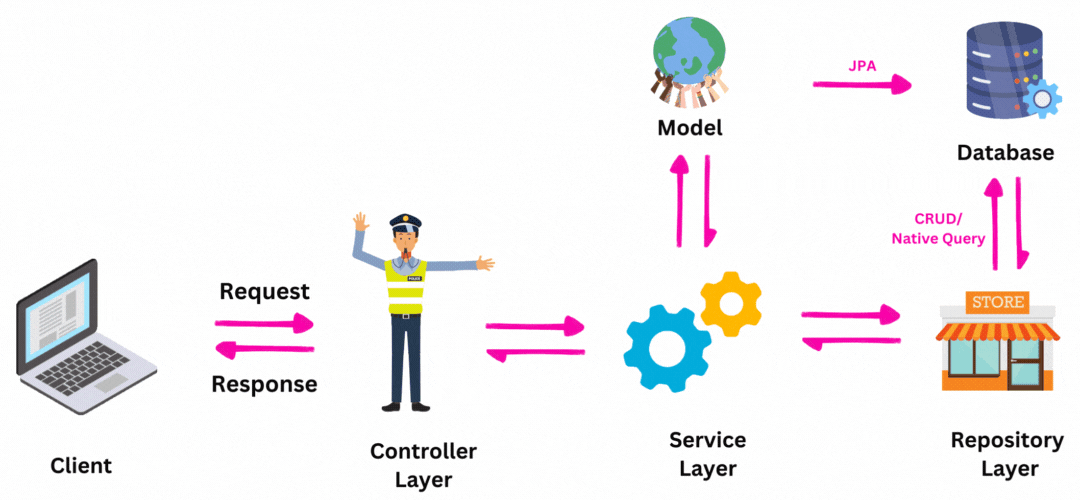
\includegraphics[width=0.75\linewidth]{imagenes/scheme/spring_boot_layers.png}
        \caption{Capas de Spring Boot hecho por \textcite{spring-layers}}
        \label{fig:spring_boot_layers}
    \end{figure}



Spring Boot se integra fácilmente con otros componentes de Spring, como Spring Security y Spring Data, y se basa en las mismas buenas prácticas que han hecho de Spring un estándar en la industria del desarrollo de software. Por ejemplo, Spring Boot facilita la integración con JPA, el cual permite la persistencia de datos en bases de datos relacionales.

\subsection{ JPA }

JPA (Java Persistence API) es una especificación que simplifica la interacción con bases de datos en aplicaciones Java. Fue introducida en 2006 como parte de la plataforma \acrfull{javaee} 5 y desarrollada por Oracle. Su objetivo es facilitar el mapeo de objetos Java a tablas de bases de datos relacionales sin la necesidad de escribir SQL manualmente. Con JPA, los desarrolladores pueden centrarse en el código de negocio sin preocuparse por los detalles de la persistencia, como se ve en el artículo de \textcite{jpa-spring-integration}.

Una de las grandes ventajas de JPA es que reduce la cantidad de código repetitivo necesario para realizar operaciones \acrfull{crud} en la base de datos. 

JPA permite que los desarrolladores trabajen con objetos de dominio directamente, delegando la gestión de las transacciones y el acceso a la base de datos en el framework subyacente. En combinación con Spring Data JPA, la interacción con la base de datos se hace más sencilla y eficiente, eliminando la necesidad de escribir consultas SQL explícitas en la mayoría de los casos.

JPA se utiliza principalmente en aplicaciones que requieren una gestión compleja de datos, y su integración con Spring Boot a través de Spring Data JPA permite acelerar el desarrollo al proporcionar un enfoque estandarizado para la persistencia de datos.



\subsection{ Maven }

Maven es una herramienta de gestión de proyectos y de automatización de construcción para aplicaciones Java, desarrollada por la Apache Software Foundation y lanzada en 2004 \parencite{maven-official}.

Su principal función es gestionar las dependencias de un proyecto, es decir, todas las bibliotecas externas que el proyecto necesita para funcionar. Maven permite a los desarrolladores definir estas dependencias en un archivo \acrfull{xml} llamado pom.xml y luego descarga automáticamente las versiones correctas de estas bibliotecas desde repositorios remotos.

Una de las mayores ventajas de Maven es su capacidad para estandarizar el proceso de construcción de aplicaciones Java, independientemente del entorno en el que se desarrolle. Esto asegura que los proyectos construidos con Maven sean consistentes y que se puedan replicar fácilmente en cualquier máquina de desarrollo.

En este proyecto, Maven juega un papel crucial al manejar las dependencias de Spring Boot, JPA y Thymeleaf, asegurando que todas las bibliotecas necesarias estén disponibles y configuradas correctamente.

\subsection{ Thymeleaf }
\label{subsec:thymeleaf}

Thymeleaf es un motor de plantillas para aplicaciones Java, creado por Daniel Fernández en 2011, que permite la generación dinámica de contenido HTML, XML y otros formatos de texto, tal y como lo explican sus creadores en la web oficial \textcite{thymeleaf-official}.

Thymeleaf se usa principalmente para construir la vista (view) o plantilla (template) en aplicaciones web, y es altamente compatible con Spring, ya que facilita la integración de los modelos de datos Java con las plantillas HTML de manera eficiente.

Una de las principales ventajas de Thymeleaf es que permite crear plantillas que pueden ser previsualizadas sin necesidad de ejecutar la aplicación en un servidor. Esto lo hace particularmente útil para el desarrollo colaborativo entre diseñadores y programadores, ya que los archivos HTML son completamente editables desde el lado del cliente.

Thymeleaf está diseñado para funcionar bien con Spring MVC y Spring Boot, lo que lo convierte en una opción natural para las aplicaciones web que necesitan generar contenido dinámico basado en datos proporcionados por el servidor.


    



    
\section{Ciberseguridad}
\label{sec:ciberseguridad}

La ciberseguridad es un aspecto crítico en el desarrollo de aplicaciones modernas, especialmente cuando se manejan datos sensibles como credenciales de usuarios, información personal, contraseñas y documentos privados. En este apartado, se describen las tecnologías y prácticas más relevantes en el ámbito de la ciberseguridad, con un enfoque en el cifrado de datos y las capas de seguridad en el proceso de autenticación.

El cifrado es una técnica fundamental para proteger la confidencialidad e integridad de los datos. Consiste en transformar la información en un formato ilegible para cualquier persona que no posea la clave de descifrado adecuada. A continuación, se describen los principales enfoques y tecnologías utilizadas en el cifrado de datos.

\subsection{Cifrado simétrico}

El cifrado simétrico \parencite{symmetric-encryption} utiliza una única clave para cifrar y descifrar los datos. Este enfoque es eficiente en términos de rendimiento, ya que requiere menos recursos computacionales en comparación con el cifrado asimétrico. Sin embargo, la gestión segura de la clave es un desafío, ya que debe compartirse entre las partes que necesitan cifrar y descifrar los datos.

 AES (\emph{Advanced Encryption Standard}) es uno de los algoritmos de cifrado simétrico más utilizados y seguros. AES opera en bloques de 128 bits y admite claves de 128, 192 o 256 bits. Su fortaleza radica en su resistencia a ataques criptográficos y su eficiencia en términos de velocidad.
 
  AES puede utilizarse en diferentes modos de operación, como \acrfull{ecb}, \acrfull{cbc} y \acrfull{gcm}. Cada modo tiene sus propias características y niveles de seguridad.


\subsection{Cifrado asimétrico}

El cifrado asimétrico, también conocido como cifrado de clave pública, utiliza un par de claves: una clave pública para cifrar los datos y una clave privada para descifrarlos. Este enfoque es ideal para escenarios donde la clave no puede compartirse de manera segura, como en la comunicación entre dos partes que no han establecido previamente una relación de confianza.

 \acrfull{rsa} es uno de los algoritmos de cifrado asimétrico más populares. RSA se basa en la dificultad de factorizar números grandes en sus componentes primos. Aunque es seguro, su rendimiento es inferior al cifrado simétrico, por lo que se utiliza principalmente para cifrar claves o datos pequeños.
   
 \emph{Curvas Elípticas} \acrfull{ecc} es una alternativa más moderna y eficiente a RSA. ECC ofrece un nivel de seguridad similar con claves más cortas, lo que reduce el consumo de recursos y mejora el rendimiento.


\subsection{Cifrado de contraseñas}

El cifrado de contraseñas es un caso especial donde se utilizan funciones de hash unidireccionales para almacenar las contraseñas de manera segura. A diferencia del cifrado tradicional, el hash no puede revertirse, lo que garantiza que incluso si la base de datos es comprometida, las contraseñas no puedan recuperarse.

\begin{itemize}
    \item BCrypt: Es una función de hash diseñada específicamente para contraseñas. BCrypt utiliza un valor de \emph{salt} \parencite{salt} único para cada contraseña, lo que aumenta la seguridad frente a ataques de diccionario y fuerza bruta. Además, su diseño permite ajustar la complejidad del hashing, lo que lo hace resistente a los avances en hardware.
    \item Argon2: Es una función de hash moderna que ha ganado popularidad debido a su resistencia a ataques de fuerza bruta y su capacidad para utilizar múltiples recursos del sistema (\acrshort{cpu}, memoria y paralelismo). Argon2 es considerado uno de los algoritmos más seguros para el cifrado de contraseñas.
\end{itemize}

\subsection{Capas de Seguridad en el login}
\label{subsec:capas-seguridad-login}

El proceso de autenticación es uno de los puntos más vulnerables en cualquier aplicación, ya que es el primer paso para acceder a los recursos protegidos. Para garantizar la seguridad del login, es esencial implementar múltiples capas de seguridad que protejan contra ataques comunes y refuercen la integridad del sistema.


Los ataques de fuerza bruta intentan adivinar las credenciales de un usuario probando múltiples combinaciones de nombres de usuario y contraseñas. Para proteger contra estos ataques, es esencial implementar medidas como:

\begin{itemize}
    \item Límite de Intentos: Bloquear temporalmente la cuenta después de un número determinado de intentos fallidos. Esto dificulta que un atacante pueda probar múltiples combinaciones en un corto período de tiempo.
    \item CAPTCHA: Requerir que el usuario resuelva un desafío \acrshort{captcha} después de varios intentos fallidos. Esto ayuda a distinguir entre usuarios legítimos y bots automatizados.
\end{itemize}

Los ataques \acrfull{csrf} explotan la confianza que un sitio web tiene en el navegador del usuario para realizar acciones no autorizadas. Para prevenir estos ataques, se pueden implementar las siguientes medidas:

\begin{itemize}
    \item Tokens CSRF: Generar un token único para cada sesión de usuario y validarlo en cada solicitud. Esto garantiza que la solicitud proviene de una fuente legítima.
    \item SameSite Cookies: Configurar las cookies con el atributo SameSite para evitar que se envíen en solicitudes cruzadas entre sitios.
\end{itemize}


El registro y monitoreo de la actividad del usuario es esencial para detectar y responder a posibles amenazas de seguridad. Algunas prácticas recomendadas incluyen:

\begin{itemize}
    \item Registro de Accesos: Registrar todos los intentos de login, tanto exitosos como fallidos, para identificar patrones sospechosos.
    \item Alertas de Seguridad: Configurar alertas para notificar a los administradores en caso de actividades inusuales, como múltiples intentos fallidos de login desde diferentes ubicaciones.
\end{itemize}


\section{Diseño software}
El diseño de software es una fase crítica en el desarrollo de aplicaciones, ya que define la estructura, organización y comportamiento del sistema. Un buen diseño no solo garantiza que el software cumpla con los requisitos funcionales, sino que también facilita su mantenimiento, escalabilidad y reutilización. En este apartado, se abordarán los patrones de diseño más comunes y los diagramas \acrfull{uml}, herramientas esenciales para modelar y documentar sistemas de software.

\subsection{Patrones de diseño software}
Los patrones de diseño son soluciones probadas y reutilizables para problemas comunes en el desarrollo de software. Estos patrones proporcionan un enfoque estructurado para resolver desafíos específicos, mejorando la calidad del código y facilitando su mantenimiento. Para más información se puede obtener el libro de \textcite{design-patterns}. A continuación, se describen algunos de los patrones más utilizados:


El patrón Fachada es un patrón estructural que proporciona una interfaz simplificada para un conjunto de interfaces en un subsistema. Este patrón es útil cuando un sistema es complejo y tiene múltiples componentes, ya que oculta la complejidad detrás de una interfaz única y fácil de usar. Por ejemplo, en una aplicación con múltiples servicios y bibliotecas, una fachada puede actuar como un punto de entrada único, reduciendo la dependencia entre los componentes y facilitando su uso.


El patrón Singleton es un patrón creacional que garantiza que una clase tenga una única instancia y proporciona un punto de acceso global a esa instancia. Este patrón es útil cuando se necesita un único punto de control, como en la gestión de configuraciones, conexiones a bases de datos o registros de logs. Al garantizar que solo exista una instancia, se evita la duplicación de recursos y se asegura un comportamiento consistente en toda la aplicación.


Además de los mencionados, existen otros patrones ampliamente utilizados, como:
\begin{itemize}
    \item Patrón Observador (Observer): Permite que un objeto notifique a otros objetos sobre cambios en su estado.
    \item Patrón Estrategia (Strategy): Define una familia de algoritmos, encapsula cada uno de ellos y los hace intercambiables.
    \item Patrón Inyección de Dependencias (Dependency Injection): Facilita la gestión de dependencias entre componentes, promoviendo un código más modular y testeable.
\end{itemize}

\subsection{Diagramas UML}
El Lenguaje Unificado de Modelado (UML, por sus siglas en inglés) es un estándar utilizado para visualizar, especificar, construir y documentar sistemas de software. Los diagramas UML son una herramienta esencial para comunicar el diseño del software entre desarrolladores, analistas y stakeholders. A continuación, se describen los tipos de diagramas más relevantes.

Muchos artículos hablan del diagrama de secuencia UML como \textcite{uml-secuence-article}. Estos explican que el diagrama de secuencia es un tipo de diagrama de interacción que muestra cómo los objetos interactúan en un escenario específico a lo largo del tiempo. Este diagrama es especialmente útil para modelar el flujo de mensajes entre objetos en un sistema, lo que permite entender cómo se ejecutan las operaciones y en qué orden.

\begin{itemize}
    \item Actores: Representan los roles externos que interactúan con el sistema, como usuarios o sistemas externos.
    \item Objetos: Representan las instancias de clases o componentes del sistema.
    \item Mensajes: Representan las interacciones entre objetos, mostrando el flujo de control y datos.
    \item Línea de vida: Muestra la existencia de un objeto durante el tiempo de ejecución.
\end{itemize}

Los diagramas de secuencia son ideales para modelar casos de uso complejos, como procesos de autenticación, transacciones o flujos de trabajo. Además, son una herramienta valiosa para identificar cuellos de botella y optimizar el rendimiento del sistema.

Además del diagrama de secuencia, UML incluye otros tipos de diagramas, como:
\begin{itemize}
    \item Diagrama de clases: Muestra la estructura estática del sistema, incluyendo clases, atributos, métodos y relaciones.
    \item Diagrama de casos de uso: Representa las interacciones entre los actores y el sistema, describiendo las funcionalidades desde la perspectiva del usuario.
    \item Diagrama de actividades: Modela el flujo de trabajo o procesos de negocio, mostrando las actividades y decisiones involucradas.
    \item Diagrama de componentes: Muestra la organización física del sistema, incluyendo módulos, bibliotecas y dependencias.
\end{itemize}

En resumen, los patrones de diseño y los diagramas UML son herramientas fundamentales en el desarrollo de software moderno. Los patrones de diseño proporcionan soluciones reutilizables para problemas comunes, mientras que los diagramas UML facilitan la comunicación y documentación del diseño del sistema. Juntos, permiten crear aplicaciones robustas, mantenibles y escalables.
